
%(BEGIN_QUESTION)
% Copyright 2006, Tony R. Kuphaldt, released under the Creative Commons Attribution License (v 1.0)
% This means you may do almost anything with this work of mine, so long as you give me proper credit

Tegn grafen til utgangen på denne regulatoren. Den har en $K_p$ på 3 og bias satt til 45\%

%Graph the output of this proportional-only controller, assuming a gain ($K_p$) value of 2.0, a bias value of 50\%, and a control action that is direct-acting:

$$\includegraphics[width=15.5cm]{i01468x01.eps}$$

\vskip 20pt \vbox{\hrule \hbox{\strut \vrule{} {\bf Suggestions for Socratic discussion} \vrule} \hrule}

\begin{itemize}
\item{} Explain why this trend graph of the PV is unrealistic for a real process, but nevertheless useful for learning how a proportional-only controller is designed to respond to changes in PV.
\item{} How do you suppose the PV would {\it actually} respond in a real process to the conditions shown (or implied) in this trend?  Sketch what you would think would be a more realistic response assuming a properly-tuned proportional-only controller running in automatic mode.
\end{itemize}

\underbar{file i01468}
%(END_QUESTION)





%(BEGIN_ANSWER)

$$\includegraphics[width=15.5cm]{i01468x02.eps}$$

%(END_ANSWER)





%(BEGIN_NOTES)


\vfil \eject

\noindent
{\bf Summary Quiz:}

The process controller generating the output seen on this trend is configured for:

$$\includegraphics[width=15.5cm]{i01468x03.eps}$$

\begin{itemize}
\item{} Direct control action
\vskip 5pt 
\item{} A proportional band value of 100\%
\vskip 5pt 
\item{} A gain value of 1.5
\vskip 5pt 
\item{} A proportional band value of 15\%
\vskip 5pt 
\item{} A gain value of 0.5
\vskip 5pt 
\item{} A proportional band value of 400\%
\end{itemize}



%INDEX% Control, proportional: graphing controller response

%(END_NOTES)


